\documentclass{article}
\usepackage{graphicx}
\usepackage{amsmath}
\usepackage[margin=3cm]{geometry}

\begin{document}

\title{The Error Function}
\author{Jens S. K. Jensen}
\date{\today}
\maketitle

\section{Introduction}
In mathematics, the error function (also called the Gauss error function) is a special function (non-elementary) of sigmoid shape that occurs in probability, statistics, and partial differential equations describing diffusion. It is defined as:
\begin{align}
	\text{erf}(x) &= \frac{2}{\sqrt{\pi}} \int_0^x e^{-t^2}\;dt \\
	&= \frac{2}{\sqrt{\pi}} \int_0^x e^{-t^2}\;dt
	\label{eq:ana}
\end{align}
In statistics, for nonnegative values of x, the error function has the following interpretation: for a random variable Y that is normally distributed with mean 0 and variance 0.5, erf(x) describes the probability of Y falling in the range [−x, x]. There are several closely related functions, such as the complementary error function, the imaginary error function, and others.

\section{Numerical solution}
The error function can also be found numerically by solving the following differential equation:
\begin{equation}
	u'(x) = \frac{2}{\sqrt{\pi}}e^{-x^2}
	\label{eq:num}
\end{equation}
with the initial condition
\begin{equation}
	u(0) = 0
	\label{eq:init}
\end{equation}

\section{Plot visualization}

Both the analytical and numerical solutions are shown in figure \ref{fig:plot}. The analytical solution (gsl erf(x)) is GSL's implementation of equation \ref{eq:ana}, while the numerical solution (myerf(x)) is computed by integrating equation \ref{eq:num} with \ref{eq:init}.

\begin{figure}[t]
	\centering
	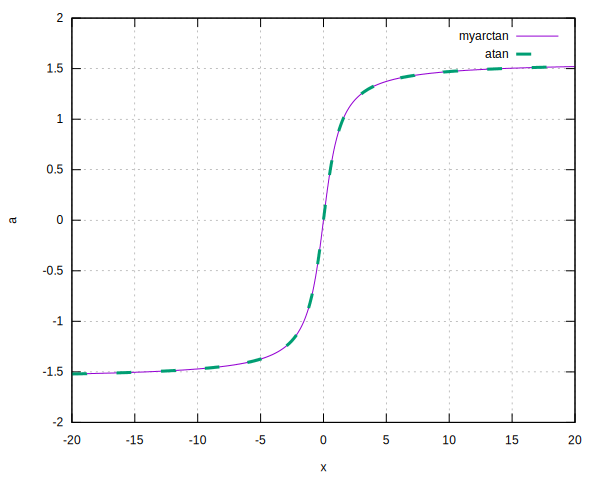
\includegraphics{plot.pdf}
	\caption{Numerical and analytical representations of the error function.}
	\label{fig:plot}
\end{figure}

\end{document}
